A lot of probability questions are in the form of ``\textsl{What is the probability of X if Y?}''
So we want to try and formulate this question mathematically.

The idea is that if we know $Y$ (where $Y$ is some event), then we can think of $Y$ as the new sample space.
Then the probability of $X$ would be the probability of $X\cap Y$ divided by the probability of $Y$.

The rationale behind this may become more clear with the following illustration:

\begin{center}
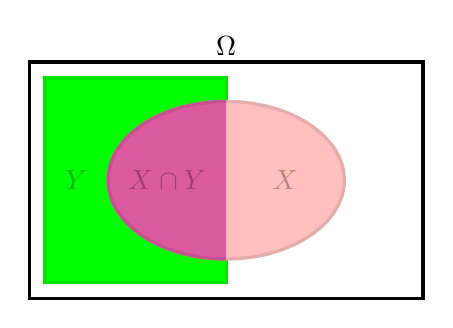
\begin{tikzpicture}

	\draw[black, very thick] (0,0) rectangle (5,3);
	\node at (2.5,3.2) {$\Omega$};

	\def\RB{(0.2,0.2) rectangle (2.5,2.8)}
	\def\CA{(2.5,1.5) ellipse (1.5 and 1)}

	\filldraw[fill=green, draw=green!90!black, very thick] \RB;
	\filldraw[fill=pink, draw=pink!90!black, very thick] \CA;

	\node[color=green!70!black] at (0.6,1.5) {$\boldsymbol Y$};
	\node[color=pink!70!black] at (3.25,1.5) {$\boldsymbol X$};

	\begin{scope}
		\clip \RB;
		\definecolor{hotpink}{RGB}{220,90,160}
		\filldraw[fill=hotpink, draw=hotpink!90!black, very thick] \CA;
		\node[color=hotpink!70!black] at (1.75,1.5) {$\boldsymbol{X\cap Y}$};
	\end{scope}

\end{tikzpicture}
\end{center}

We want to focus our attention on $X\cap Y$ within $Y$.

\begin{defn*}

	If $\tuple{\Omega,\cF,\prob}$ is a probability space, and $B$ is an event in $\cF$ such that $\probof B>0$,
	we define the \ppemph{conditional probability function} of $B$ to be a function:
	\[ \probof{\;\cdot}[B]\colon\cF\longrightarrow[0,1] \]
	Where $\probof{A}[B]$ is defined as:
	\[ \probof{A}[B]\coloneqq\frac{\probof{A\cap B}}{\probof B} \]

	Another notation for $\probof{A}[B]$ is $\probof[B]{A}$.

\end{defn*}

\begin{prop*}[bayesLaw,Baye's\ Law]

	\[ \probof{A}[B] = \probof{B}[A] \cdot \frac{\probof A}{\probof B} \]

\end{prop*}

\begin{proof}

	This is quite simple, notice:
	\[ \probof{A}[B] = \frac{\probof{A\cap B}}{\probof B} =
	\frac{\probof{A\cap B}}{\probof{A}}\cdot\frac{\probof A}{\probof B} = \probof{B}[A]\cdot\frac{\probof A}{\probof B} \]
	As required.

\hfill$\qed$

\end{proof}

\begin{thrm*}[totProbTwoTheorem,Law\ of\ Total\ Probability\ Version\ Two]

	If $\set{A_i}_{i\in I}\in\cF$ is a countable partition of $\Omega$, and for every $i\in I$, $\probof{A_i}>0$,
	then for every event $B\in\cF$:
	\[ \probof{B} = \sum_{i\in I}\probof{B}[A_i]\cdot\probof{A_i} \]

\end{thrm*}

\begin{proof}

	By the \ppref{totProbOneTheorem}, we know:
	\[ \probof{B} = \sum_{i\in I}\probof{B\cap A_i} \]
	And since $\probof{B\cap A_i} = \probof{B}[A_i]\cdot\probof{A_i}$, we see:
	\[ \probof{B} = \sum_{i\in I}\probof{B}[A_i]\cdot\probof{A_i} \]
	As required.

\hfill$\qed$

\end{proof}

\begin{lemm*}

	If $A$, $B$, and $C$ are events, such that $\probof{B},\probof{C}>0$, then:
	\[ \prob\parens{A \;\middle|\; B \;\middle|\; C} = \probof{A}[B\cap C] \]

\end{lemm*}

\begin{proof}

	We know:
	\[ \prob\parens{A \;\middle|\; B \;\middle|\; C} = \probof[C]{A}[B] = \frac{\probof[C]{A\cap B}}{\probof[C]{B}}
	   = \frac{\probof{A\cap B\cap C} / \probof{C}}{\probof{B\cap C} / \probof{C}}
	   = \frac{\probof{A\cap B\cap C}}{\probof{B\cap C}} \]
	And on the other hand, we know:
	\[ \probof{A}[B\cap C] = \frac{\probof{A\cap B\cap C}}{\probof{B\cap C}} \]
	As required.

\hfill$\qed$

\end{proof}

\begin{thrm*}

	If $\set{A_i}_{i=1}^n\in\cF$ are events, then:
	\[ \probof{\bigcap_{i=1}^n A_i} = \prod_{i=1}^n\probof{A_i}[\bigcap_{j=1}^{i-1}A_j] \]

	This is the mathematical concept behind the commonly taught ``tree method'' for computing the probability of
	intersections.

	When $i=1$, we must define $\bigcap_{j=1}^{i-1}A_j=\Omega$, since conditional probability is not defined on $\varnothing$,
	as it has zero probability.

\end{thrm*}

\begin{proof}

	We will prove this through induction on $n$.

	\ppemph{Base case:} $n=1$.

	Then the product is equal to simply:
	\[ \probof{A_1}[\Omega] = \probof{A_1} \]
	As required.

	\ppemph{Base case:} $n=2$

	So we need to show that:
	\[ \probof{A_1\cap A_2} = \probof{A_1}\cdot\probof{A_2}[A_1] \]
	And this is true by the definition of conditional probability.

	\ppemph{Inductive step:}
	We know:
	\[ \probof{\bigcap_{i=1}^{n+1}A_i} = \probof{\bigcap_{i=1}^{n-1}A_i \cap (A_n\cap A_{n+1})} \]
	Which is equal to, by our inductive hypothesis:
	\[ = \prod_{i=1}^{n-1}\probof{A_i}[\bigcap_{j=1}^{i-1}A_j] \cdot \probof{A_n\cap A_{n+1}}[\bigcap_{j=1}^{n-1}A_j] \]
	And by our base case for $n=2$, we know that:
	\begin{align*}
		\probof{A_n\cap A_{n+1}}[\bigcap_{j=1}^{n-1}A_j] &= \probof{A_n}[\bigcap_{j=1}^{n-1}A_j] \cdot
		\probof{A_{n+1}\;\middle|\; A_n}[\bigcap_{j=1}^{n-1}A_j] \\ &= \probof{A_n}[\bigcap_{j=1}^{n-1}A_j] \cdot
		\probof{A_{n+1}}[\bigcap_{j=1}^n A_j]
	\end{align*}
	So all in all:
	\[ \probof{\bigcap_{i=1}^{n+1}A_i} = \prod_{i=1}^{n-1}\probof{A_i}[\bigcap_{j=1}^{i-1}A_j] \cdot
	   \probof{A_n}[\bigcap_{j=1}^{n-1}A_j] \cdot \probof{A_{n+1}}[\bigcap_{j=1}^n A_j] \]
	And this is just equal to:
	\[ = \prod_{i=1}^{n+1}\probof{A_i}[\bigcap_{j=1}^{i-1}A_j] \]
	As required.

\hfill$\qed$

\end{proof}

\begin{defn*}

	Two events, $A$ and $B$, are \ppemph{independent}if $\probof{A\cap B}=\probof{A}\cdot\probof{B}$.

	This is denoted as $A\indep B$.

\end{defn*}

It is worth noting that independence is symmetric: if $A$ and $B$ are independent, $B$ and $A$ are independent.
This is because intersection and multiplication is commutative.

\begin{prop*}

	The following are equivalent:
	\begin{msecenumerate}
		\mitem $A$ and $B$ are independent.
		\mitem $\probof{A}[B]=\probof{A}$
		\mitem $\probof{B}[A]=\probof{B}$
	\end{msecenumerate}

\end{prop*}

\begin{proof}

	\vskip -\baselineskip
	\begin{multiparitemize}[0pt]
		\paritem{\alphabull{1\implies2}} We know that:
			\[ \probof{A}[B] = \frac{\probof{A\cap B}}{\probof{B}} = \frac{\probof A\cdot\probof B}{\probof B} = \probof A \]
			As required.
		\paritem{\alphabull{2\implies 3}} By \ppref{bayesLaw} we know:
			\[ \probof{B}[A] = \probof{A}[B]\cdot\frac{\probof B}{\probof A} = \probof A\cdot\frac{\probof B}{\probof A} =
			\probof B \]
			As required.
		\paritem{\alphabull{3\implies1}} We know:
			\[ \probof{B} = \frac{\probof{B\cap A}}{\probof{A}} \implies \probof{A\cap B}=\probof{A}\cdot\probof{B} \]
			Which means $A$ and $B$ are independent, as required.
	\end{multiparitemize}

\hfill$\qed$

\end{proof}

\begin{prop*}

	\begin{msecenumerate}[0pt]
		\mitem If $\probof A$ is equal to $0$ or $1$ if and only if for every $B\in\cF$, $A\indep B$.
		\mitem An event $A$ is independent of every every event if and only if it is independent of itself.
		\mitem If $A$ and $B$ are disjoint events with non-zero probability, they are not independent.
		\mitem If $A$ is a subset of $B$, $\probof A\neq0$, and $\probof B\neq1$, then $A$ and $B$ are not independent.
		\mitem If $A$ and $B$ are independent, so are $A^c$ and $B$.
	\end{msecenumerate}

\end{prop*}

\begin{proof}

	\vskip -\baselineskip
	\begin{msecenumerate}[0pt]
		\mitem $(\boldsymbol\implies)$ Suppose $\probof A=0$.
			Since $A\cap B\subseteq A$, that means $\probof{A\cap B}\leq\probof{A}=0$, so $\probof{A\cap B}=0$.
			And since $\probof{A}\cdot\probof{B}=0\cdot\probof B=0$, $\probof{A\cap B}=\probof A\cdot\probof B$, as required.

			Now suppose $\probof A=1$.
			We know then that $\probof{A^c}=0$.
			We also know that:
			\[ \probof{A\cap B} = 1-\probof{A^c\cup B^c} \]
			By the union bound, $\probof{A^c\cup B^c}\leq\probof{A^c}+\probof{B^c}=\probof{B^c}$.
			But on the other hand, since $B^c\subseteq A^c\cup B^c$, $\probof{B^c}\leq\probof{A^c\cup B^c}$, so
			$\probof{A^c\cup B^c}=\probof{B^c}$.

			Therefore:
			\[ \probof{A\cap B} = 1 - \probof{B^c} = \probof{B} = \probof{A}\cdot\probof{B} \]
			As required.

			$(\boldsymbol\impliedby)$ Since $A$ is independent of every event, it must be independent of itself, so:
			\[ \probof{A} = \probof{A\cap A} = \probof{A}^2 \]
			This means that $\probof A$ is equal to $0$ or $1$, as required.

		\mitem As shown in the above proof, $A$ is independent of itself if and only if $\probof A$ is $0$ or $1$.
			And by above, this is equivalent to $A$ being independent of every event.

		\mitem Since $A\cap B=\varnothing$, $\probof{A\cap B}=0$.
			But $\probof{A},\probof B>0$, so $\probof A\cdot\probof B\neq0$, so $A$ and $B$ are dependent.

		\mitem Since $A\subseteq B$, $\probof{A\cap B}=\probof{A}$.
			This equal to $\probof A\cdot\probof B$ if and only if $\probof A=0$ or $\probof B=1$, which they don't.

		\mitem We know
			\[ \probof{A^c\cap B} = \probof{B} - \probof{A\cap B} =
			   \probof B - \probof A\cdot\probof B = \probof B(1-\probof A) = \probof{A^c}\cdot\probof B \]
			As required.

			\begin{note}
				Using this, we can show that $A\indep B$, $A^c\indep B$, $A\indep B^c$, and $A^c\indep B^c$ are all
				equivalent.
			\end{note}
	\end{msecenumerate}

\end{proof}

\begin{defn*}

	A set of events, $\set{A_i}_{i=1}^n$ is independent if for every set $I\subseteq[n]$:
	\[ \probof{A_I} = \prod_{i\in I}\probof{A_i} \]

	(Recall that $A_I=\bigcap\limits_{i\in I}A_i$.)

	And for an arbitrary indexing set $I$, $\set{A_i}_{i\in I}$ is independent if for every finite subset $J\subset I$,
	$\set{A_j}_{j\in J}$ is independent.

\end{defn*}

\begin{prop*}

	Suppose $\set{A_i}_{i=1}^\infty$ is independent, then:
	\[ \probof{\bigcap_{i=1}^\infty A_i} = \prod_{i=1}^\infty\probof{A_i} \]

\end{prop*}

\begin{proof}

	Let:
	\[ B_m\coloneqq\bigcap_{i=1}^m A_m \]
	Which means that:
	\[ \bigcap_{m=1}^\infty B_m = \bigcap_{m=1}^\infty A_m \]

	Furthermore, we know that $B_m$ must be decreasing as $B_{m+1}=B_m\cap A_{m+1}$.
	Therefore, by \ppref[theorem]{contProbTheorem}, we know that:
	\[ \lim_{m\to\infty}\probof{B_m} = \probof{\bigcap_{i=1}^\infty B_i} \]
	And by the definition of $B_m$, this means
	\[ \lim_{m\to\infty}\probof{\bigcap_{i=1}^m A_i} = \probof{\bigcap_{i=1}^\infty A_i} \]
	Since $\set{A_i}_{i=1}^\infty$ is independent:
	\[ \lim_{m\to\infty}\probof{\bigcap_{i=1}^m A_i} = \lim_{m\to\infty}\prod_{i=1}^m \probof{A_i} =
	   \prod_{i=1}^\infty\probof{A_i} \]
	
	So:
	\[ \probof{\bigcap_{i=1}^\infty A_i} = \prod_{i=1}^\infty\probof{A_i} \]
	As required.

\hfill$\qed$

\end{proof}

\begin{defn*}

	Suppose $\set{B_i}_{i=1}^n$ is a set of events, and $A$ is some other event.
	We say that $A$ is independent of $\set{B_i}_{i=1}^n$ if for every set $I\subseteq[n]$, $A$ and $B_I$ are independent.

\end{defn*}

\begin{prop*}

	Suppose $\set{A_i}_{i=1}^n$ is a set of events.
	Then $\set{A_i}_{i=1}^n$ is independent if and only if every $A_j$ is independent of 
	$\set{A_i}_{i=1}^n\setminus\set{A_j}$.

\end{prop*}

\begin{proof}

	$(\boldsymbol\implies)$ Let $I\subseteq[n]$ such that $j\notin I$.
	We must show that $A_j$ and $A_I$ are independent.
	We know that:
	\[ \probof{A_j\cap A_I} = \probof{A_{I\cup\set{j}}} = \prod_{i\in I}\probof{A_i} \cdot\probof{A_j} =
	   \probof{A_I}\cdot\probof{A_j} \]
	As required.

	$(\boldsymbol\impliedby)$ Suppose $I=\set{i_1,\dots,i_k}\subseteq[n]$.
	Then:
	\[ \probof{A_I} = \probof{A_{i_1}\cap A_{I\setminus\set{i_1}}} \]
	Since $A_{i_1}$ is independent of $A_{I\setminus\set{i_1}}$, this is equal to:
	\[ = \probof{A_{i_1}} \cdot \probof{A_{I\setminus\set{i_1}}} \]
	And then using induction on the size of $I$, we get that this is equal to:
	\[ = \probof{A_{i_1}} \cdot \prod_{i\in I\setminus\set{i_1}}\probof{A_i} = \prod_{i\in I}\probof{A_i} \]
	So $\set{A_i}_{i=1}^n$ is independent.

\hfill$\qed$

\end{proof}

\begin{defn*}

	A set $\set{A_i}_{i=1}^n$ is \ppemph{pairwise independent} if for every relevant $i\neq j$, $A_i$ and $A_j$ are
	independent.

\end{defn*}

\begin{note}

	If a set is independent, it is also pairwise independent.
	This is since you can take the set $\set{i,j}$.

	But the reverse is not true.
	This can be demonstrated with the following example:

	\def\bx{\boldsymbol x}
	Suppose we flip a coin $k$ times, where $k$ is odd.
	Our sample space $\Omega$ will be the set of all vectors $\bx\in[0,1]^k$ which
	correspond to the result of the flips ($\bx_i$ is the result of the $i$th flip, $1$ is heads, etc.).
	Let's define the following events for all $i\in[k]$:
	\[ A_i = \set{\bx\in\Omega}[\bx_i=1] \]
	And:
	\[ B = \set{\bx\in\Omega}[\sum_{i=1}^k\bx_i\equiv 0\pmod{2}] \]
	($A_i$ is the event that the $i$th flip resulted in heads, $B$ is the event that there is an even amount of heads.)


	Notice that the probability of $A_i$ and the probability of $B$ are both $\frac12$ (by symmetry), and:
	\[ A_i\cap B = \set{\bx}[\bx_1+\cdots+\bx_{i-1}+1+\bx_{i+1}\cdots+\bx_k\equiv0\pmod{2}] =
	   \set{\bx}[\sum_{\substack{j=1\\j\neq i}}\bx_j\equiv1\pmod{2}]\cap\set{\bx}[\bx_i=1] \]
	Both of these events are independent and have probability $\frac12$, so the probability $\probof{A_i\cap B}=\frac14$.
	So $A_i$ and $B$ are independent.
	Furthermore, $A_i$ and $A_j$ are independent (this is trivial).
	So the set $\set{A_1,\dots,A_k,B}$ is pairwise independent.

	But:
	\[ A_{[k]}\cap B = \set{\bx}[\forall i\in{[k]}: \bx_i=1, \sum_{i=1}^k\bx_i\equiv0\pmod2] =
	   \set{\bx}[\bx_i=1, k\equiv0\pmod2] \]

	But since $k$ is odd, $k\not\equiv0\pmod2$, so the set is the empty set and therefore has probability $0$.
	But $A_i$ and $B$ don't, so $\set{A_1,\dots,A_k,B}$ is not independent.

\end{note}

